% 2008 年湖北卷文科第 18 题：直三棱柱 ABC-A1B1C1，平面 A1BC ⊥ 侧面 A1ABB1。
% 来源 PDF：gaokaomath-src/普通高考/2008/2008湖北文.pdf
% SHA-256：e097163e244cb8f03775ac7ff2e344ef85471e91ecc717d23698a0fb01e76963
% 原页：2008湖北文.pdf 第 2 页（A3 三栏）第 1 栏，书页码 452。
% 重绘依据：按原页斜投影：上底 A1（左上）、C1（右上）、B1（右中），下底 A（左下）、C（右下）、
%   B（下中）；可见棱 A1C1、A1B1、B1C1、AA1、BB1、CC1、AB、BC 与对角 A1B 实线，
%   A—C 为被遮挡的底边（虚线）。
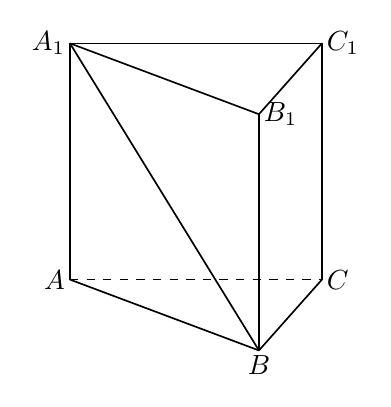
\begin{tikzpicture}[scale=1.0, semithick, every node/.style={inner sep=1.5pt}]
  \coordinate (A) at (0.20,0.40);
  \coordinate (C) at (3.40,0.40);
  \coordinate (B) at (2.60,-0.50);
  \coordinate (A1) at (0.20,3.40);
  \coordinate (C1) at (3.40,3.40);
  \coordinate (B1) at (2.60,2.50);

  \draw (A1) -- (C1);
  \draw (A1) -- (B1);
  \draw (B1) -- (C1);
  \draw (A) -- (A1);
  \draw (B) -- (B1);
  \draw (C) -- (C1);
  \draw (A) -- (B);
  \draw (B) -- (C);
  \draw (A1) -- (B);
  \draw[dashed] (A) -- (C);

  \node[left] at (A) {$A$};
  \node[below] at (B) {$B$};
  \node[right] at (C) {$C$};
  \node[left] at (A1) {$A_1$};
  \node[right] at (B1) {$B_1$};
  \node[right] at (C1) {$C_1$};
\end{tikzpicture}
